\documentclass[11pt,letterpaper]{article}
\usepackage[utf8]{inputenc}
\usepackage[T1]{fontenc}
\usepackage[english]{babel}
\usepackage{lmodern}
\usepackage{amsmath,amssymb,amsfonts}
\usepackage[margin=2.5cm]{geometry}
\usepackage{fancyhdr}
\usepackage{enumitem}
\usepackage[most]{tcolorbox}
\usepackage{xcolor}
\usepackage{tikz}
\usetikzlibrary{arrows.meta,angles,quotes,calc,babel}
\usepackage{placeins}
\usepackage{needspace}

% ============ PALETTE: BLACK, ORANGE, AND CREAM ============
\definecolor{blackmain}{HTML}{1A1A1A}
\definecolor{orangeacc}{HTML}{E65C00}
\definecolor{creambg}{HTML}{FBF8F1}
\definecolor{orangebg}{HTML}{FFF4EB}
\definecolor{graymuted}{HTML}{7A746E}
\definecolor{pureblack}{HTML}{0D0D0D}

% ============ HEADERS AND FOOTERS ============
\setlength{\headheight}{24pt}
\pagestyle{fancy}
\fancyhf{}
\fancyhead[L]{\textcolor{blackmain}{\textbf{\small Mathematical Methods I}}}
\fancyhead[R]{\textcolor{orangeacc}{\textbf{\small Directional Derivative}}}
\fancyfoot[C]{\textcolor{graymuted}{\thepage}}
\renewcommand{\headrulewidth}{0.8pt}
\renewcommand{\headrule}{\hbox to\headwidth{\color{orangeacc}\leaders\hrule height \headrulewidth\hfill}}

\setlist[itemize]{label={\small\textcolor{orangeacc}{$\blacksquare$}},leftmargin=1.6em}
\setlist[enumerate]{label={\textcolor{orangeacc}{\arabic*.}},leftmargin=1.8em}

% ============ TITLES ============
\newcommand{\manualsection}[1]{%
  \Needspace{16\baselineskip}%
  \vspace{0.35cm}
  \par\noindent{\Large\bfseries\color{blackmain} #1}\par\nobreak
  \noindent{\color{orangeacc}\rule{\linewidth}{1.4pt}}\par\nobreak
  \vspace{0.15cm}
}

\newcommand{\manualsubsection}[1]{%
  \par\vspace{0.2cm}\noindent{\bfseries\color{orangeacc} #1}\par\nobreak
  \vspace{0.12cm}
}

% ============ CONTENT BOXES ============
\newtcolorbox{infobox}[2][orangeacc]{
  enhanced,
  colback=creambg,colframe=#1!90!black,
  boxrule=1pt,arc=2mm,
  left=9pt,right=9pt,top=8pt,bottom=8pt,
  before upper={\textbf{\color{#1!95!black}\large #2}\par\nobreak
    {\color{#1!50}\rule{\linewidth}{0.6pt}}\par\nobreak\smallskip}
}

\newtcolorbox{examplebox}[1]{
  enhanced,
  colback=orangebg,colframe=orangeacc!85!black,
  boxrule=1pt,arc=2mm,
  left=9pt,right=9pt,top=8pt,bottom=8pt,
  before upper={\textbf{\color{orangeacc!95!black}\large #1}\par\nobreak
    {\color{orangeacc!40}\rule{\linewidth}{0.6pt}}\par\nobreak\smallskip}
}

\newtcolorbox{theorembox}[1]{
  enhanced,
  colback=creambg!70!white,colframe=pureblack,
  boxrule=1.1pt,arc=2mm,
  left=9pt,right=9pt,top=8pt,bottom=8pt,
  before upper={\textbf{\color{pureblack}\large #1}\par\nobreak
    {\color{orangeacc}\rule{\linewidth}{0.8pt}}\par\nobreak\smallskip}
}

\newcommand{\term}[1]{\textbf{\color{orangeacc}#1}}
\newcommand{\termb}[1]{\textbf{\color{blackmain}#1}}
\renewcommand{\familydefault}{\rmdefault}
\tikzset{every node/.append style={font=\rmfamily}}

\begin{document}
\color{blackmain}

\begin{center}
  {\LARGE\textbf{\color{blackmain}Mathematical Methods I}}\\[0.2cm]
  {\Large\textcolor{orangeacc}{\textbf{Directional Derivatives and Vector Fields}}}\\[0.4cm]
  {\large\textcolor{graymuted}{Gabriel Velázquez}}\\[0.35cm]
\end{center}

\manualsection{1. Derivative with Respect to a Tangent Vector}

A \term{directional derivative} measures the instantaneous rate of change of a scalar
function as one moves in a given direction. It generalizes partial derivatives:
these describe change along the coordinate axes, whereas a directional derivative
allows us to consider any vector.

\begin{infobox}[orangeacc]{Definition 1.1 (Directional Derivative)}
Let $\Omega\subseteq\mathbb{R}^n$ be an open set, $p\in\Omega$, and
$\mathbf{v}\in\mathbb{R}^n$. The \term{tangent vector} $\mathbf{v}_p$ is the
vector $\mathbf{v}$ based at the point $p$. For $f:\Omega\to\mathbb{R}$, define
\begin{equation}
  \mathbf{v}_p[f]
  =\left.\frac{d}{dt}f(p+t\mathbf{v})\right|_{t=0}
  =\lim_{t\to0}\frac{f(p+t\mathbf{v})-f(p)}{t},
\end{equation}
provided the limit exists. This is also written as $D_{\mathbf{v}}f(p)$.
\end{infobox}

The curve $\gamma(t)=p+t\mathbf{v}$ traces a straight line when
$\mathbf{v}\neq\mathbf{0}$, with $\gamma(0)=p$ and velocity
$\gamma'(0)=\mathbf{v}$. Thus, $\mathbf{v}_p[f]$ is the ordinary derivative
of the single-variable function $f\circ\gamma$ at $t=0$.

\begin{figure}[htbp]
\centering
\begin{tikzpicture}[scale=0.95,>=Stealth]
  \draw[->,graymuted] (0,0)--(6.4,0) node[right] {$x_1$};
  \draw[->,graymuted] (0,0)--(0,2.9) node[above] {$x_2$};
  \coordinate (P) at (1.4,0.8);
  \coordinate (Q) at (4.2,2.0);
  \draw[dashed,graymuted] (0.35,0.35)--(5.6,2.6);
  \draw[->,orangeacc,very thick] (P)--(Q)
    node[midway,above left] {$\mathbf{v}_p$};
  \fill[blackmain] (P) circle (2pt) node[below right] {$p$};
  \node[blackmain,below right] at (Q) {$p+\mathbf{v}$};
  \node[orangeacc,above] at (4.8,2.7) {$\gamma(t)=p+t\mathbf{v}$};
\end{tikzpicture}
\caption{The derivative is evaluated at $p$ along the line with velocity $\mathbf{v}$.}
\label{fig:directional-path}
\end{figure}
\FloatBarrier

\newpage
\manualsection{2. Computation in Cartesian Coordinates}

\begin{theorembox}{Theorem 2.1 (Coordinate Formula)}
If $f:\Omega\to\mathbb{R}$ is differentiable at $p$ and
$\mathbf{v}=(v_1,\ldots,v_n)$, the chain rule gives
\begin{equation}
  \mathbf{v}_p[f]
  =\sum_{i=1}^{n}v_i\frac{\partial f}{\partial x_i}(p)
  =\nabla f(p)\cdot\mathbf{v}.
\end{equation}
In particular, in $\mathbb{R}^3$,
\begin{equation}
  \mathbf{v}_p[f]
  =v_1\frac{\partial f}{\partial x_1}(p)
   +v_2\frac{\partial f}{\partial x_2}(p)
   +v_3\frac{\partial f}{\partial x_3}(p).
\end{equation}
Here $\nabla f(p)$ is the \term{gradient}: the vector of partial derivatives of $f$
evaluated at $p$.
\end{theorembox}

The differentiability assumption is important: the mere existence of partial
derivatives at $p$ is not enough to justify this formula.

\manualsubsection{Direction and Speed}
$\mathbf{v}_p[f]$ is defined for a vector of any length;
it measures change per unit of the parameter $t$. To measure change
per unit distance in the direction of $\mathbf{v}\neq\mathbf{0}$, use
the unit vector $\widehat{\mathbf{v}}=\mathbf{v}/\|\mathbf{v}\|$:
\begin{equation}
  D_{\widehat{\mathbf{v}}}f(p)
  =\frac{\mathbf{v}_p[f]}{\|\mathbf{v}\|}.
\end{equation}

\begin{examplebox}{Example 2.2 (Evaluation at a Point)}
Let $f(x,y,z)=x^2y+z^2$, $p=(1,2,-1)$, and $\mathbf{v}=(2,-1,3)$.
Then
\[
  \nabla f(x,y,z)=(2xy,x^2,2z),
  \qquad \nabla f(p)=(4,1,-2).
\]
Therefore,
\[
  \mathbf{v}_p[f]=4(2)+1(-1)+(-2)(3)=1.
\]
This can be verified directly along the line:
\[
  f(p+t\mathbf{v})
  =(1+2t)^2(2-t)+(-1+3t)^2
  =3+t+13t^2-4t^3.
\]
Its derivative at $t=0$ is $1$. Since $\|\mathbf{v}\|=\sqrt{14}$, the derivative
in the corresponding unit direction is $1/\sqrt{14}$.
\end{examplebox}

\newpage
\manualsection{3. Properties of the Directional Derivative}

Let $f,g:\Omega\to\mathbb{R}$ be differentiable at $p$, let
$\mathbf{v}_p,\mathbf{w}_p$ be tangent vectors at the same point, and let
$a,b\in\mathbb{R}$ be constants. The directional derivative satisfies
the usual rules of differentiation.

\begin{theorembox}{Theorem 3.1 (Linearity)}
\termb{Linearity in the function:}
\begin{equation}
  \mathbf{v}_p[af+bg]=a\,\mathbf{v}_p[f]+b\,\mathbf{v}_p[g].
\end{equation}
\termb{Linearity in the vector:}
\begin{equation}
  (a\mathbf{v}_p+b\mathbf{w}_p)[f]
  =a\,\mathbf{v}_p[f]+b\,\mathbf{w}_p[f].
\end{equation}
The second identity follows from the linearity of the differential
$df_p(\mathbf{v})=\nabla f(p)\cdot\mathbf{v}$. It applies to vectors without
normalizing them after addition.
\end{theorembox}

\begin{theorembox}{Theorem 3.2 (Product Rule or Leibniz Rule)}
\begin{equation}
  \mathbf{v}_p[fg]
  =\mathbf{v}_p[f]\,g(p)+f(p)\,\mathbf{v}_p[g].
\end{equation}
The undifferentiated factors are evaluated at the base point $p$.
\end{theorembox}

\begin{theorembox}{Theorem 3.3 (Chain Rule)}
If $h:\mathbb{R}\to\mathbb{R}$ is differentiable at $f(p)$, then
\begin{equation}
  \mathbf{v}_p[h\circ f]=h'(f(p))\,\mathbf{v}_p[f].
\end{equation}
This follows by differentiating $h(f(p+t\mathbf{v}))$ with respect to $t$ at $t=0$.
\end{theorembox}

\begin{examplebox}{Example 3.4 (Applying the Rules)}
For $f$, $p$, and $\mathbf{v}$ from Example 2.2, $f(p)=3$ and
$\mathbf{v}_p[f]=1$. By the chain rule,
\[
  \mathbf{v}_p[f^2]=2f(p)\,\mathbf{v}_p[f]=6.
\]
If, in addition, $g(x,y,z)=x+z$, then $g(p)=0$ and
$\mathbf{v}_p[g]=2+3=5$. The Leibniz rule yields
\[
  \mathbf{v}_p[fg]=1(0)+3(5)=15.
\]
\end{examplebox}

\newpage
\manualsection{4. Vector Fields as Operators}

A \term{vector field} $V$ assigns a tangent vector $V(p)$ to each point
$p\in\Omega$. Unlike a fixed vector $\mathbf{v}_p$, which acts at a single point,
the field allows us to differentiate a function at every point of its domain.

\begin{infobox}[orangeacc]{Definition 4.1 (Action of a Field on a Function)}
For a differentiable function $f:\Omega\to\mathbb{R}$, the expression $V[f]$
denotes the new \term{scalar function} defined by
\begin{equation}
  (V[f])(p)=V(p)[f].
\end{equation}
If $V(p)=(v_1(p),\ldots,v_n(p))_p$, then
\begin{equation}
  (V[f])(p)=\sum_{i=1}^{n}v_i(p)\frac{\partial f}{\partial x_i}(p).
\end{equation}
As an identity between functions, this is written as
\begin{equation}
  V[f]=\sum_{i=1}^{n}v_i\frac{\partial f}{\partial x_i}.
\end{equation}
\end{infobox}

\begin{theorembox}{Theorem 4.2 (Properties of the Operator $V$)}
For differentiable functions $f,g$, constants $a,b\in\mathbb{R}$, and a scalar
function $\phi$ defined on $\Omega$,
\begin{align}
  V[af+bg]&=aV[f]+bV[g],\\
  V[fg]&=V[f]g+fV[g],\\
  (\phi V)[g]&=\phi\,V[g].
\end{align}
In the last identity, $\phi$ multiplies the field: it is not differentiated.
In contrast, $V[\phi g]=V[\phi]g+\phi V[g]$ when $\phi$ is differentiable.
\end{theorembox}

\begin{examplebox}{Example 4.3 (From a Number to a Function)}
In $\mathbb{R}^2$, let $V(x,y)=(y,-x)_{(x,y)}$ and $f(x,y)=x^2y$. Then
\[
  V[f](x,y)=y(2xy)-x(x^2)=2xy^2-x^3.
\]
The result is a function of $(x,y)$. A number is obtained only after evaluating
it at a point: for $p=(1,2)$,
\[
  (V[f])(p)=7=V(p)[f],\qquad V(p)=(2,-1)_p.
\]
\end{examplebox}


\begin{figure}[htbp]
\centering
\begin{tikzpicture}[scale=0.85,>=Stealth]
  \draw[step=1,graymuted!15] (-2.7,-2.7) grid (2.7,2.7);
  \draw[->,graymuted] (-3,0)--(3.2,0) node[right] {$x$};
  \draw[->,graymuted] (0,-3)--(0,3.2) node[above] {$y$};
  \foreach \xx in {-2,-1,0,1,2} {
    \foreach \yy in {-2,-1,0,1,2} {
      \fill[graymuted] (\xx,\yy) circle (1pt);
      \pgfmathtruncatemacro{\nonzero}{abs(\xx)+abs(\yy)}
      \ifnum\nonzero>0
        \draw[->,orangeacc,thick] (\xx,\yy)--++({0.32*\yy},{-0.32*\xx});
      \fi
    }
  }
  \fill[blackmain] (1,2) circle (2.2pt)
    node[above=3pt] {$p$};
  \draw[->,blackmain,very thick] (1,2)--(1.64,1.68);
  \draw[graymuted] (1.7,1.75)--(3.4,2.3);
  \node[anchor=west,align=left] at (3.5,2.3)
    {$V(p)=(2,-1)_p$\\[-1pt]\small A vector based at $p=(1,2)$};
  \node[anchor=west,align=left] at (3.5,0.5)
    {$V(x,y)=(y,-x)_{(x,y)}$\\[4pt]
     \small Direction: clockwise\\
     \small Length: $\|V(x,y)\|=\sqrt{x^2+y^2}$};
  \node[anchor=west,align=left] at (3.5,-1.5)
    {$V(0,0)=\mathbf{0}_{(0,0)}$\\[-1pt]\small The field vanishes at the origin};
\end{tikzpicture}
\caption{A vector field assigns a vector to every point. For the field in
Example 4.3, the vectors are tangent to circles centered at the origin and
grow in length with the distance from it. All arrows use the same reduced
scale; the highlighted arrow represents the vector at $p$.}
\label{fig:vector-field}
\end{figure}
\FloatBarrier

\newpage
\manualsection{5. The Natural Frame and Partial Derivatives}

In Cartesian coordinates, the fields of the \term{natural frame}
$U_1,\ldots,U_n$ assign the standard basis vectors to each point:
$U_i(p)=(\mathbf{e}_i)_p$. In $\mathbb{R}^3$,
\[
  U_1(p)=(1,0,0)_p,\qquad
  U_2(p)=(0,1,0)_p,\qquad
  U_3(p)=(0,0,1)_p.
\]

\begin{infobox}[blackmain]{Proposition 5.1 (Natural Fields and Partial Derivative Operators)}
For every differentiable function $f$,
\begin{equation}
  U_i[f]=\frac{\partial f}{\partial x_i}.
\end{equation}
In particular, using coordinates $(x,y,z)$,
\[
  U_1[f]=\frac{\partial f}{\partial x},\qquad
  U_2[f]=\frac{\partial f}{\partial y},\qquad
  U_3[f]=\frac{\partial f}{\partial z}.
\]
Through its action on functions, $U_i$ is identified with the operator
$\partial/\partial x_i$.
\end{infobox}

Every vector field can be expressed uniquely in terms of its coordinate functions:
\begin{equation}
  V=\sum_{i=1}^{n}v_iU_i
  =\sum_{i=1}^{n}v_i\frac{\partial}{\partial x_i}.
\end{equation}
Applying this expression to $f$ gives:
\begin{equation}
  V[f]=\left(\sum_{i=1}^{n}v_iU_i\right)[f]
  =\sum_{i=1}^{n}v_iU_i[f]
  =\sum_{i=1}^{n}v_i\frac{\partial f}{\partial x_i}.
\end{equation}
The coefficients are functions, not necessarily constants. For the coordinate
functions, $U_i[x_j]=\delta_{ij}$ and hence $V[x_j]=v_j$;
this recovers each component and explains uniqueness.

\begin{examplebox}{Example 5.2 (One Field, Two Notations)}
The field from Example 4.3 can be written as
\[
  V=yU_1-xU_2
   =y\frac{\partial}{\partial x}-x\frac{\partial}{\partial y}.
\]
Thus, $V[x]=y$, $V[y]=-x$, and $V[x^2y]=2xy^2-x^3$.
\end{examplebox}


\begin{figure}[htbp]
\centering
\begin{tikzpicture}[scale=0.9,>=Stealth]
  \begin{scope}
    \draw[->,graymuted] (-0.3,0)--(5,0) node[right] {$x$};
    \draw[->,graymuted] (0,-0.3)--(0,4.4) node[above] {$y$};
    \foreach \xx in {1,3} {
      \draw[dashed,graymuted!40] (\xx,0.2)--(\xx,4);
    }
    \foreach \yy in {1,3} {
      \draw[dashed,graymuted!40] (0.2,\yy)--(4.5,\yy);
    }
    \foreach \xx in {1,3} {
      \foreach \yy in {1,3} {
        \draw[->,orangeacc,very thick] (\xx,\yy)--++(1,0);
        \draw[->,blackmain,very thick] (\xx,\yy)--++(0,1);
        \fill[blackmain] (\xx,\yy) circle (1.8pt);
      }
    }
    \node[orangeacc,below] at (3.6,3) {$U_1$};
    \node[blackmain,left] at (3,3.6) {$U_2$};
    \node[align=center,font=\small] at (2.5,-0.85)
      {The same coordinate basis\\at every point};
  \end{scope}
  \begin{scope}[xshift=8cm,yshift=1cm]
    \draw[dashed,orangeacc!60] (-1,0)--(3.2,0)
      node[right,blackmain] {$y=p_y$};
    \draw[dashed,graymuted] (0,-0.7)--(0,3.2)
      node[above,blackmain] {$x=p_x$};
    \draw[->,orangeacc,very thick] (0,0)--(2,0)
      node[midway,below=5pt] {$U_1(p)=\left.\frac{\partial}{\partial x}\right|_p$};
    \draw[->,blackmain,very thick] (0,0)--(0,2)
      node[midway,right=5pt] {$U_2(p)=\left.\frac{\partial}{\partial y}\right|_p$};
    \fill[blackmain] (0,0) circle (2pt) node[below left] {$p$};
    \node[align=center,font=\small] at (1,-1.85)
      {At $p$: differentiate along one coordinate\\while holding the other fixed};
  \end{scope}
\end{tikzpicture}
\caption{The Cartesian natural frame in $\mathbb{R}^2$. The fields
$U_1=\partial/\partial x$ (orange) and $U_2=\partial/\partial y$ (black)
are tangent to the coordinate lines and form a basis at each point.
Their action on a scalar function gives $U_1[f]=\partial f/\partial x$
and $U_2[f]=\partial f/\partial y$. The right panel enlarges one such basis.}
\label{fig:natural-frame}
\end{figure}
\FloatBarrier

\end{document}
